\documentclass[runningheads,a4paper]{llncs}

\usepackage[american]{babel}

\usepackage{graphicx}
\usepackage{amssymb}
\usepackage[utf8]{inputenc}
\usepackage[T1]{fontenc}

%extended enumerate, such as \begin{compactenum}
\usepackage{paralist}

%put figures inside a text
%\usepackage{picins}
%use
%\piccaptioninside
%\piccaption{...}
%\parpic[r]{\includegraphics ...}
%Text...

%Sorts the citations in the brackets
%\usepackage{cite}

%for easy quotations: \enquote{text}
\usepackage{csquotes}

\usepackage[T1]{fontenc}

%enable margin kerning
\usepackage{microtype}

%better font, similar to the default springer font
\usepackage[%
rm={oldstyle=false,proportional=true},%
sf={oldstyle=false,proportional=true},%
tt={oldstyle=false,proportional=true,variable=true},%
qt=false%
]{cfr-lm}
%
%if more space is needed, exchange cfr-lm by mathptmx
%\usepackage{mathptmx}

%for demonstration purposes only
\usepackage[math]{blindtext}

\usepackage{multirow}
\usepackage[table,xcdraw]{xcolor}

\usepackage[
%pdfauthor={},
%pdfsubject={},
%pdftitle={},
%pdfkeywords={},
bookmarks=false,
breaklinks=true,
colorlinks=true,
linkcolor=black,
citecolor=black,
urlcolor=black,
%pdfstartpage=19,
pdfpagelayout=SinglePage
]{hyperref}
%enables correct jumping to figures when referencing
\usepackage[all]{hypcap}

\usepackage[inline]{enumitem}


\usepackage{enumitem}
\setlist[itemize,1]{label={\fontfamily{cmr}\fontencoding{T1}\selectfont\textbullet}}

\usepackage[capitalise,nameinlink]{cleveref}
%Nice formats for \cref
\crefname{section}{Sect.}{Sect.}
\Crefname{section}{Section}{Sections}
\crefname{figure}{Fig.}{Fig.}
\Crefname{figure}{Figure}{Figures}

\usepackage{amsmath}

%Table of contents
% make a proper TOC despite llncs
\setcounter{tocdepth}{3}
\makeatletter
\renewcommand*\l@author[2]{}
\renewcommand*\l@title[2]{}
\makeatletter




\usepackage{xspace}
\usepackage{cite}
%\newcommand{\eg}{e.\,g.\xspace}
%\newcommand{\ie}{i.\,e.\xspace}
\newcommand{\eg}{e.\,g.,\ }
\newcommand{\ie}{i.\,e.,\ }

\setcounter{secnumdepth}{3}

%introduce \powerset - hint by http://matheplanet.com/matheplanet/nuke/html/viewtopic.php?topic=136492&post_id=997377
\DeclareFontFamily{U}{MnSymbolC}{}
\DeclareSymbolFont{MnSyC}{U}{MnSymbolC}{m}{n}
\DeclareFontShape{U}{MnSymbolC}{m}{n}{
    <-6>  MnSymbolC5
   <6-7>  MnSymbolC6
   <7-8>  MnSymbolC7
   <8-9>  MnSymbolC8
   <9-10> MnSymbolC9
  <10-12> MnSymbolC10
  <12->   MnSymbolC12%
}{}
\DeclareMathSymbol{\powerset}{\mathord}{MnSyC}{180}

%improve wrapping of URLs - hint by http://tex.stackexchange.com/a/10419/9075
\makeatletter
\g@addto@macro{\UrlBreaks}{\UrlOrds}
\makeatother

% correct bad hyphenation here
\hyphenation{optical networks semiconductor}

\begin{document}

%Works on MiKTeX only
%hint by http://goemonx.blogspot.de/2012/01/pdflatex-ligaturen-und-copynpaste.html
%also http://tex.stackexchange.com/questions/4397/make-ligatures-in-linux-libertine-copyable-and-searchable
%This allows a copy'n'paste of the text from the paper
\input glyphtounicode.tex
\pdfgentounicode=1

\title{Cloud Computing in Nonprofit Organizations}
%If Title is too long, use \titlerunning
%\titlerunning{Short Title}

%Single insitute
\author{Diogo André Cardoso Serafim\\
\textit{diogoserafim@tecnico.ulisboa.pt}
\\Advisor: José Borbinha 
\\Co-Advisor: Por definir}
%If there are too many authors, use \authorrunning
%\authorrunning{First Author et al.}
\institute{Instituto Superior Técnico}
\authorrunning{Cardoso Serafim et al.}


%Multiple insitutes
%Currently disabled
%
\iffalse
%Multiple institutes are typeset as follows:
\author{Firstname Lastname\inst{1} \and Firstname Lastname\inst{2} }
%If there are too many authors, use \authorrunning


\institute{
Insitute 1\\
\email{...}\and
Insitute 2\\
\email{...}
}
\fi
			
\maketitle


\begin{abstract}

\iffalse
Network security threats are becoming more and more proeminent and the connection links at ISPs are getting increasingly fast. Traditional network intrusion detection systems are either signature-based or behavior-based, which means looking up for known intrusion signatures in the packets, or detecting deviation from a normal behavior, respectively. With the exponential increase of network security threats, these IDSs are not able to cope with their growth, as they are only able to detect specific intrusions that are previously known. Also, most of them rely on payload inspection, that can be a bottleneck in the detection in real-time, and, now that almost every communication is done through encrypted messages, it is almost impossible to interpret the observed payload. In order to counter these limitations, our IDS will detect attacks using flows, which are defined as being a set of packets that passes a specific observation point in a given time period, with common characteristics. This work will therefore present a proposal for a flow-based IDS capable of detecting attacks without any \textit{a priori} knowledge, and therefore countering the limitations present in traditional IDSs. The results from this proposed system are to be validated with a real-world dataset provided by the Portuguese ISP Vodafone.
\fi

\end{abstract}

\keywords{Cloud Computing, Google, Authentication }



\tableofcontents

%%%%%%%%%%%%%%%%%%%%%%%%%%%%%%%%%%%%%%%%%%%%%%%%%%%%%%%%%%%%%%%%%%%%%%%%%%%%%%%
\section{Introduction}\label{sec:intro}
%%%%%%%%%%%%%%%%%%%%%%%%%%%%%%%%%%%%%%%%%%%%%%%%%%%%%%%%%%%%%%%%%%%%%%%%%%%%%%%

Preserving the security of a network is becoming increasingly more important nowadays. The number of security threats is growing day by day, and the networks' security systems must be able to keep up with this. Moreover, Internet Service Providers are increasing the capacity of their backbone links, now operating in the order of 1 to 10 Gbps. Traditional Intrusion Detection Systems (IDSs) usually operate by using deep packet inspection, meaning that they look up on the payload of the packets passing through specific points of the network (e.g. may be observing either edge or border router), looking for a certain signature or a certain behavior pattern. This would be feasible for link connections that were rather slow, but now it is very difficult to analyze the payload of every packet passing through the routers and be able to process them in real-time, without creating a bottleneck. Also, nowadays most of the traffic payload is sent across the network encrypted, which makes this kind of detection even harder. An alternative to this approach is the use of \textit{flows}. This concept was first suggested by Cisco, and is defined as being a sequence of packets passing through an observation point with the same features, in a given period of time. This allows to observe the communication between hosts, rather than the content of the exchange packets, opening a whole new world for Network Intrusion Detection Systems (NIDSs). Traditionally, a 5-tuple is extracted from the observed flows, being composed by the Source IP address, Destination IP address, Source Port, Destination Port and Transport Protocol. 

There are basically two main approaches when it comes to classifying an Intrusion Detection System:
\begin{enumerate*}
\item Signature-based detection
\item Behavior-based detection
\end{enumerate*}. In the former, the system looks for a certain sequence in the observed traffic in order to match it with a known intrusion; for the case of deep packet inspection, it would look in sequences of bytes in the payload in order to find a signature of a known intrusion, while when using a flow-based approach it would be, for example, to look for flows with an active SYN flag. In the case of behavior-based detection, the system first builds what would be a normal behavior profile, and then look for traffic that deviate from this profile (normally certain thresholds are imposed, as defining the limit for the acceptable behavior). 

However, these two approaches lack in generality, i.e. they are designed to detect only what is previously known, and, at the moment, most of the existing IDSs are configured either with signatures or normal behavior. Even though these may present good results, they do not scale with the increasing number of novel threats. It would be necessary to be constantly updating the system with information regarding these new kinds of attacks or intrusions.

With this work, we aim to present a flow-based Network Intrusion Detection System that is able to overcome these issues. This means creating a NIDS operating on a flow-level, that is able to detect intrusion without having \textit{a priori} knowledge of the intrusions. This can be done by using machine learning techniques to train the system, as we will further discuss. By achieving this, we have a system that provides increased autonomy and is, in a way, self-learning, which may reduce a lot of the network managers' constant need for intervention.

To achieve so, the system will first preprocess the incoming flows, filtering the network traffic, in which all traffic that is either internal or directed to a well-destination, is removed. This filtered traffic will then be fed to a clustering algorithm that will group hosts who share a same pattern. This will allow for the managers to have a better understanding of what could be corresponding to a threat. Upon this grouping, there will be a manual intervention from part of the network managers to analyze the traffic considered as outlier by the clustering algorithm, that will proceed to label it. Finally, this labeled traffic will be fed to a supervised learning algorithm that will rank it, ultimately indicating that it may or not be an intrusion. 

This document is structured as follows:
\begin{itemize}
\item Section \ref{sec:related} aims to explore some relevant studies on this field;
\item Section \ref{sec:arch} provides the proposed solution architecture;
\item Section \ref{sec:eval} provides the evaluation methods for the validation of the solution;
\item Section \ref{sec:schedule} present a scheduling for the future work;
\item Section \ref{sec:conclusion} presents some conclusions of this work.
\end{itemize}


%%%%%%%%%%%%%%%%%%%%%%%%%%%%%%%%%%%%%%%%%%%%%%%%%%%%%%%%%%%%%%%%%%%%%%%%%%%%%%%
\section{Related Work}\label{sec:related}
%%%%%%%%%%%%%%%%%%%%%%%%%%%%%%%%%%%%%%%%%%%%%%%%%%%%%%%%%%%%%%%%%%%%%%%%%%%%%%%

This section provides an overview of same major contributions in this area. Section \ref{ssec:tools} provides an insight of some of the existing tools to perform flow analysis. Section \ref{ssec:monitor} proceeds to point out some network monitoring applications that were built in a flow-based fashion. Section \ref{ssec:detection} gives an overview of some of the most addressed network intrusions and respective works that show how to detect them using a flow-level analysis rather than payload inspection. At last, Section \ref{ssec:mlearning} gives a brief explanation of what machine learning is and how it can be used to achieve our goal. 


%%%%%%%%%%%%%%%%%%%%%%%%%%%%%%%%%%%%%%%%%%%%%%%%%%%%%%%%%%%%%%%%%%%%%%%%%%%%%%
\subsection{Network Flows and Basic Flow Tools}\label{ssec:tools}
%%%%%%%%%%%%%%%%%%%%%%%%%%%%%%%%%%%%%%%%%%%%%%%%%%%%%%%%%%%%%%%%%%%%%%%%%%%%%%%

As stated previously, network flows allow a different approach in analyzing, monitoring and securing a network. While deep packet inspection allows for \textit{signature-based} approaches, making it easier to detect some kinds of attacks, its not scalable for high speed networks, e.g. 10 Gbit/s \cite{Sperotto2010} - the packets' payloads can not be analyzed in real time, for these kinds of speeds. Also, nowadays most packets exchanged have their payload encrypted, making it even more difficult to inspect, even if it was possible to process those many packets in real time. 


In 1996, Cisco developed the first network protocol to handle \textit{network flows}: NetFlow \cite{Claise2004}. This consist in a built-in software in their routers, and is used to collect and export flow records. As the years went by, new versions arrived and were more and more complete. The most recent version - NetFlow v9 - includes integration with protocols such as MPLS that were not supported in the previous versions.


Before we proceed to detail this protocol, first we must explain what a \textit{flow} is. A \textit{flow} is defined as being an unidirectional sequence of packets, passing through an observation point that satisfies a set of common features in a given period of time;  in this case, an observation point would be a Cisco NetFlow-enabled router. These features must be defined \textit{a priori}, in order for the device to perform the matching of features (an example of such features will be presented further ahead). 

Being this technology built-in in network devices, it allows to select, from all the traffic passing through that device, what we want really to analyze. For example, by deploying this in a border router, all of the traffic going in and out of that network will be filtered by NetFlow. Upon the arriving of an IP packet, the network device looks at that packet's fields in order to find any matching feature with those previously defined. In case the packet's features do match, then an entry is created in a data structure called \textit{flow cache}, for that flow. Note that a flow may contain several packets, and many different flows can be collected. This process is depicted in Figure \ref{fig:nfarch}.

As this cache cannot be kept indefinitely, certain policies were defined for its management. According to those policies, when of them is satisfied, the entries belonging to that cache will be exported to another device. So, a packet will be exported when: (i) the end of a flow if detected; (ii) a flow is inactive (i.e. when, for a given timeout, there are no longer packets belonging to a flow); (iii) belonging to a long-lasting flow, the timeout is reached; (iv) the device is in need of resources, e.g. internal memory.   


\begin{figure}[htp]
\centering
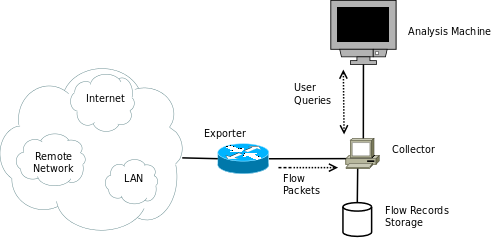
\includegraphics[scale=0.70]{netflow_arch.png}
\caption{A typical NetFlow architecture}
\label{fig:nfarch}
\end{figure}


The device to which the flow records are exported is referred to as the \textit{Collector}, and is physically located in another device. In order to achieve maximum efficiency latency-wise, these records are encapsulated in an UDP datagram. However, NetFlow also provides the possibility of exporting the data through SCTP (Stream Control Transport Protocol), if we want to operate in a congestion-aware environment.


However, this technology initially did not have in consideration any security issue - no confidentiality, integrity or authentication is guaranteed. This was designed as such due to efficiency and scalability issues - the deployment of such technology in large networks would no be able to provide real time measures. Instead, it assumed that the exporters (and also collectors) are deployed within a private, restricted and controlled network, rather than a public network, in which anyone could sniff these records, or even forge them.


Apart from NetFlow, many other vendors have their own implementation for flow collection and exporting. Examples of such implementations are NetFlow-lite, sFlow, NetStream, etc.


Due to the heterogeneous nature of this technologies from each of the vendors existing in this market, the Internet Engineering Task Force (IETF) joined forces to create a standard in flow collection and exportation, thus allowing for the clients to easily deploy their flow-based applications. This protocol was given the name IPFIX (IP Flow Information eXport) \cite{Claise2013}. As previously stated, packets who share common properties are grouped in flows, and in the IPFIX terminology they are referred to as \textit{flow keys}, and these can be, for example a tuple such as:


\emph{(IP\_source, IP\_destination, port\_source, port\_destination, typeOfService)}


In NetFlow, the flow exportation was done by  encapsulating the records into UDP or SCTP datagrams. IPFIX provides, in addition to these protocols, the option of exporting flow records through TCP. Also, it fills the security gap in Cisco's implementation: IPFIX provides both confidentiality, integrity, and authentication. These three properties are guaranteed by using secure channels - either through TLS (Transport Layer Security), if the records are exported through TCP, or through DTLS (Datagram Transport Layer Security) if the records are to be exported through UDP or SCTP datagrams. Furthermore, X.509 Certificates are also used, in order to reinforce the latter property.

In order to simplify the implementation of these frameworks, there are some tools available. Such is the case of \textit{nfdump} \cite{nfdump}, compatible with versions v5 v7 and v9 of NetFlow. It consists of six built-in functions:
\begin{itemize}
\item \textit{nfcapd}, used to read the collected NetFlow data and store it into files
\item \textit{nfdump}, used to read the files generated by the previous function, displays the data and its able to create statistics on it
\item \textit{nfprofile}, also reads the data from the generated file, and filters it according to the user define profile, storing it into a file
\item \textit{nfreplay}, which reads the data from the file generated by \textit{nfcapd} and sends it to another host
\item \textit{nfclean.pl}, a script to cleanup out of date data
\item \textit{ft2nfdump}, used to convert other flow tools data into \textit{nfdump} format
\end{itemize} 

Although this is a command line based tool, there is a graphical web-based front-end application, made to provide a better view over the gathered data.


Another tool, that is widely deployed, is SiLK - System for Internet-Level Knowledge \cite{silk}, a flow analysis tool developed by the CERT Network Situational Awareness Team. As stated in the official documentation, its ideal application is for traffic analysis on the backbone of a large enterprise or mid-sized ISPs. It is compatible with both IPFIX and NetFlow (versions v5 and v9). 


This tool is divided in two categories of applications: 
\begin{enumerate*}
\item a packing system
\item an analysis suite
\end{enumerate*}. Upon the arrival of a flow record, the packing system converts that data into another format (so that it can be more easily processed by this tool) and saves this newly converted data into a binary file. From the new data, the analysis suite, which consists of small functions to read the generated file, can perform many operations that can go from filtering to statistical analysis of the records:
\begin{itemize}
\item \textit{rwfilter}, which filters the gathered data, according to the specified conditions
\item \textit{rwcut}, which is able to convert the binary flow data contained in the generated file into a format that is perceptible by the human analyst
\item \textit{rwstats}, that generates the aforementioned statistical data
\item \textit{rwcount}, that summarizes the whole network traffic
\end{itemize}


%%%%%%%%%%%%%%%%%%%%%%%%%%%%%%%%%%%%%%%%%%%%%%%%%%%%%%%%%%%%%%%%%%%%%%%%%%%%%%%
\subsection{Flow-based Network Monitoring}\label{ssec:monitor}
%%%%%%%%%%%%%%%%%%%%%%%%%%%%%%%%%%%%%%%%%%%%%%%%%%%%%%%%%%%%%%%%%%%%%%%%%%%%%%%
Amongst many other applications, such as the monitoring of applications, hosts, security, account and billing, the analysis of network flows has been widely deployed for network monitoring. In this subsection we refer some of the existing work done in this area.


\cite{schatzmann2011fact} presented a flow-based network monitoring system called FACT - Flow-based Approach for Connectivity Tracking. Their goal was to deliver a monitoring system focused on remote hosts and networks, and to check if they are reachable from inside their (network operators) network or a costumer's network, and to trigger an alarm in case there are any kinds of connectivity problems. Such problems could be for example an unusually high number of outgoing connection from the inside of the network to remote host (which could indicate an ongoing \textit{port scan}).


First of, their flow collection was retrieved from \textit{all} network border routers, in order to inspect every single packet that leaves or enters the network. Also, the flow traffic was divided in 5 different classes, namely \textit{Traversing}, representing that traffic that comes from outside the network, passes through it and leaves, \textit{InOut}, the traffic that goes outside and returns, \textit{OnlyOut}, the traffic that only leaves the network, \textit{OnlyIn}, the traffic that comes from outside specifically to the inside of the network, and \textit{Internal}, the traffic that circulates inside the network, without leaving it. However, as this work's goal was to monitor the availability of the connection to remote hosts and networks from the inside of the network, the traffic classes \textit{Traversing} and \textit{OnlyIn} were ignored in this process, and a special focus was given to \textit{OnlyOut}. Also, there is a basic assumption that where flow is considered complete, i.e. for each outgoing flow there must be an incoming reply to that same flow.

In order to identify the critical events, connection-wise, they aggregate \textit{OnlyOut} flows types across external hosts, /24 networks and prefixes observed in public BGP tables, and then they take into account the number of affected internal hosts. After this data collecting there is a pre-processing of the data, where there is a removal of some flows (e.g. blacklisted hosts) as a filtering for the flow cache where the data will actually processed, and will stay for a period of 5 minutes. When in the flow cache, the flows are stored as a tuple containing the IP addresses, the application ports and the protocol numbers. When the 5 period minute expires, the flows are divided in two groups:
\begin{enumerate*}
\item \textit{ConnSuccess} if the bidirectional \textit{OnlyOut} flows start or end within the timeout interval (5 minutes) and they were initiated by an internal host
\item \textit{ConnFailed}, which includes only unidirectional \textit{OnlyOut} flows that either end or start within the timeout interval
\end{enumerate*}. This way, they were able to identify which remote hosts or network were totally unreachable from the inside of the network, and providing the network managers an easy way to visualize and interpret the ongoing occurrences in the network.


Another possible usage of flow-based models in network monitoring is to diagnose backbone links for network operators, or Internet Service Providers, for instance. A work in this line is \cite{sukhov2009active}. In order to do so, they use a simple flow-based model to check for active flows in the network and identify the quality of their connection, making it possible to know when a link needs an upgrade. 


Their flow-based model relies on an existing Poisson shot-noise model (a type of electric noise that can be modeled with the Poisson processes, and whose application can be, for example, the modeling of network traffic \cite{kluppelberg1995explosive}). With the use of the following three parameters, its able to make an approximation of the throughput of the backbone link: $ \lambda $ - the arrival rate of flows, $ E[S_{n}] $ - the average size of a flow, and $ E[S_{n}^2 / D_{n}] $ - the average value for the ratio of the square of a flow size and its duration. Also, it allows to characterize the data rate existing in a backbone link, with the following input: 
\begin{enumerate*}
\item session arrivals for any period where the traffic intensity is nearly constant, and are accurately modeled by a homogeneous Poisson process of finite rate $ \lambda $ (which lasts for approximately 30 minutes)
\item distribution of the flow sizes and their durations (which are independent)
\item the flow rate function
\end{enumerate*}
. Based on these values, it is possible to determine the total rate of data in the link at a given time $ t $, and consequently its average total traffic and variance. However, if such value is calculated in function of the average size of the flow, that function is only applicable to the ideal case of a backbone link with infinite capacity, and that's never achievable in a real network. So, in order to acquire the real network state, Little's Law is used, and such is given by $ N = \lambda E[D_{n}] $, where $ N $ is the mean of active network flows.

They analyzed the connection quality at the backbone link by investigating graphical dependencies between the link utilization and the number of active flows, i.e. a graphic in which the $ x $ axis represents the number of active flows and the $ y $ axis represents the link utilization. They managed to observe that there are three real network states: the first is called the operational region, and corresponds to a nearly ideal behavior, as the link utilization grows linearly with the number of active flows; the second is when the network starts getting moderately loaded and diverging from the ideal behavior; the first and last state is when the network is completely disabled, and the packet losses begin, as well as the decrease of its throughput. Also, they presented a an equation which allows to obtain a good confidence interval, based on the the flow performance, the standard deviation of the link utilization and a parameter $ \alpha $ obtained from data processing. 

These theoretical models were evaluated through experiments made from two different networks, with a data set consisting of data collected every 30 minutes throughout a week (for the first network) and every 5 minutes throughout 72 hours (for the second network). With this model, they were able to diagnose the backbone link, and check when the link utilization was beginning to leave the operation region, making possible to the network managers to know when to upgrade the link's capacity, and to steadily dimension the connections.  



A study on the effects of DDoS attacks on network flow monitoring applications is reported in \cite{Sadre2012}. Their goal was to show how a flow monitoring reacts in the the presence of such an attack. The proposed scenario was a traditional flow-based setup, where all the traffic in the network is filtered by an exporter placed in an \textit{observation point} (a Cisco NetFlow-enabled router). It then proceeds to export the collected packets with its flow records to a device in charge of generating flow records - the Collector - which, on its turn, redirects these records to the monitoring application (a already described in the previous section). They break down their approach in two parts: they first studied the impact of the attack in the flow exporter (the monitoring probe), and then they study the impacts on the flow monitoring application.

Due to the great number of flow records generated by DDoS attacks, a strategy to manage the flow record cache must be chosen. Upon the arrival of a new flow record, one of three actions can be taken: 
\begin{enumerate*}
  \item prematurely export the stored records
  \item directly export the new record
  \item prevent flow from being created
\end{enumerate*}, being the first one elected. As a consequence, there will be an increase in the rate of exported flow records, both for normal and attack traffic. Not only the rate will increase, but also, as the records have a smaller lifetime, these flows will have fewer packets - this is due to the fact that this DDoS attack consists in flooding the network with SYN Request, and each one of these requests creates a new unique flow. One other result of such decision is that, since the rate of exportation rises, there is a decrease in the delay between flow expiration and flow exportation.

Then, they used a simple single queuing model in order to study to effects on the flow monitoring application. All of the following work and conclusions was based on three assumptions: 
\begin{enumerate*}
  \item the exporter is not a bottleneck in the system
  \item the network connection between exporter and collector is well dimensioned
  \item incoming records are buffered by the application, if needed
\end{enumerate*}. This queue operates in a FIFO fashion, and each job represents a flow packet, which, in its turn, only carries the number of normal and attack flow records. They point out to the fact that if such a system is not sufficiently well dimensioned, such an attack could easily overload it: if the service rate $ \mu $ is much smaller than the arrival rate $ \lambda $, the systems is easily flooded. Furthermore, they effective rate of processed flows is a function of the rate arrival rate o attack records, and not only the normal ones. This means that during an attack, the normal flow traffic is also affected, which means that, for our case, the development of an IDS, it might be interesting to also analyze the "normal" traffic in order to detect suspicious activity. 




%%%%%%%%%%%%%%%%%%%%%%%%%%%%%%%%%%%%%%%%%%%%%%%%%%%%%%%%%%%%%%%%%%%%%%%%%%%%%%%
\subsection{Intrusion Detection based on Network Flows}\label{ssec:detection}
%%%%%%%%%%%%%%%%%%%%%%%%%%%%%%%%%%%%%%%%%%%%%%%%%%%%%%%%%%%%%%%%%%%%%%%%%%%%%%%

Nowadays, there are numerous numbers of existing network attacks. From simple port or network scans to complex botnet infrastructures, there are numerous types of different attacks, both in type, in scale or severity of impact. However, as the variety of the attacks is indeed enormous, we can not focus on the detection of all of them. Moreover, a flow-based intrusion detection approach is not able to detect all kinds of attacks, as it relies on the inspection of header information. Logic attacks such as \textit{buffer overflows} and \textit{SQL injections} can only be detected by inspecting the payload of the packets in the network, which represents a major limitation if one is to use an exclusively flow-based IDS.


With the help of some of the technologies and tools referred in Section \ref{ssec:tools}, we present some approaches on the detection of these attacks, namely \textit{port scans}, \textit{denial of service}, \textit{worms} and \textit{botnets}  


%%%%%%%%%%%%%%%%%%%%%%%%%%%%%%%%%%%%%%%%%%%%%%%%%%%%%%%%%%%%%%%%%%%%%%%%%%%%%%%
\subsubsection{Port Scanning}
%%%%%%%%%%%%%%%%%%%%%%%%%%%%%%%%%%%%%%%%%%%%%%%%%%%%%%%%%%%%%%%%%%%%%%%%%%%%%%%

A \textit{port scan} is defined as the act of consistently probing a target host (which may be either a single machine or an entire network - \textit{network scan}), by sending a large amount of generally small packets. 

This attack is generally the first step of almost every network attack (such is the case in \textit{DoS/DDoS}, \textit{worms} and \textit{botnets}), thus being its detection a crucial step for a Network IDS. As the attacker sends a great number of packets, even though these may be very small, it will produce many flows, therefore making it possible to rely on flow-based approach to detect it, as it can be very easily addressed. \cite{Northcutt} divides this attack in three distinct categories:

\begin{itemize}
	\item \textit{Horizontal scan}, in which a single host scans multiple ports in a single machine
	\item \textit{Vertical scan}, in which a single host scans one single port in multiple machines
	\item \textit{Block scan}, a combination of the two scans above -  a single host scanning multiple ports in multiple machines
\end{itemize}

Whatever category the attack falls in, this may create an anomaly in the normal network traffic pattern, and many kinds of different flows can be observed. 

Most of these attacks are investigated by observing a flow characteristic that registers the most significant difference when compared to normal traffic: the unusually high number of incoming and outgoing connections in a host. This is due to the fact that the attacker, or attackers, probe many different ports and machines, therefore generating an anomalous amount of new flows.

A type of attack that falls into this category is the brute-force SSH network attack \cite{Hellemons2012}. This is a particularly interesting attack in this field of study. The attack consists in three phases (that will be explained better further ahead): it begins by consistently scanning a certain number of victim, until a running port is found; then, it attempts to login in those victims through a brute-force dictionary attack; once it gains access, the attacker can do whatever it wants with the victim, and also to others that might belong to the same network. Therefore, SSH attacks can be potential harmful not only to hosts individually, but also to the network it is connect to. 

However, the detection of these attacks, as they rely mainly on \textit{scanning}, can be address by performing an analysis of the network traffic at a flow-level. \cite{Hellemons2012} presented a flow-based Intrusion Detection System called \textit{SSHCure}, which allows for real-time detection of brute-force SSH network attacks. 

Their solution was based on the observation made by \cite{Northcutt}. They observed that the behavior of the attacks over time, in terms of flows, follows a pattern of evolution, and it can be identified in three distinct phases, as described below:

\begin{enumerate}
	\item Scanning phase, in which the attacker performs a \textit{port scan} for a certain IP address block, in order to find running SSH daemons in a host (SSH daemons use TCP port 22)
	\item Brute-force phase, in which the attackers tries to login to a certain number of hosts, by means of a dictionary attack - various combinations of usernames and passwords
	\item Die-off phase, in which after successfully login into the victim host, the traffic volume is drastically reduced, leaving only residual traffic
\end{enumerate}


By tracking these three phases in a flow pattern, this attack can easily be identified. Moreover, \cite{kim2004flow} also proposed a solution to detect this intrusion by, once again observing flow-based traffic patterns. This approach will be explained in more detail in the next section.

%%%%%%%%%%%%%%%%%%%%%%%%%%%%%%%%%%%%%%%%%%%%%%%%%%%%%%%%%%%%%%%%%%%%%%%%%%%%%%%
\subsubsection{Denial of Service}
%%%%%%%%%%%%%%%%%%%%%%%%%%%%%%%%%%%%%%%%%%%%%%%%%%%%%%%%%%%%%%%%%%%%%%%%%%%%%%%
A \textit{Denial of Service} (\textit{DoS}), is the attempt of an attacker to make a certain server, firewall, or even a whole network unable to reply, by flooding it with several requests and thus draining all of its resources. In a DoS attack there is generally one single attacker. This has some limitation to the attacker, such as the fact that it may not scale when targeting a big number of victims, or even the fact the if one single attacker is producing all the traffic, it is easier to detect, due to the large anomalous volume of traffic. Another kind of DoS attacks is the Distributed Denial of Service, in which now there as various sources that are producing this large volume of traffic, thus making it more difficult to detect, as the traffic is now more evenly distributed and hidden (this was already discussed in Section \ref{ssec:monitor}).

According to Peng \textit{et al.} \cite{Peng2007} and Kim \textit{et al.} \cite{kim2004flow}, there can be various types of DoS/DDoS attacks:


\begin{itemize}
\item \emph{SYN flood} - this attack aims to explore the vulnerability the \textit{three-way handshake}, the connection establishment procedure in the TCP protocol. As depicted in Figure \ref{fig:handshake}, to establish a TCP session, the one initiating the connection (the client) will send a packet with an activive SYN flag, to which the entity on the other end (the server) replies with a SYN/ACK flagged packet. The session is successfully established when the client replies to the latter packet with one that has an ACK flag. Whenever a client initiates the three-way handshake, the server will store this request information in its memory, and will keep it until it receives an acknowledge. Usually, in these attacks, the attacker sends packets with an active SYN flag and an nonexistent IP source address, therefore making the server unable to respond with the SYN/ACK packet; this can also be done with a source that exists, but that machine has to be configured such that they ignore any correspondent packet originated from the server. By send multiple packets with active SYN flags, the server's memory will be exhausted, and be unable to respond to any other requests


\item \emph{ICMP flood} - this attack is labeled as a bandwidth attack, as its goal is to congest the communication channels in a network. When a broadcast message in sent, there will be as many packets being sent in the network as the number of connected hosts; by sending multiple broadcast messages, the bandwidth can easily be depleted


\item \emph{Smurf} - this attack consists in sending an ICMP Echo Request packet whose destination source is the broadcast address of a network. Also, the source address is external to the compromised network and is propagated with the use of intermediates (who can also be victims in this attack)

\item \emph{Fraggle} - this attacks is performed is performed like the \textit{Smurf} attacks, except now the UDP protocol is used, instead of ICMP

\item \emph{Ping of Death} - this attacks consists in sending multiple (e.g. thousands per second) spoofed pings with an abnormally large size
 
\item \emph{Land} - this attacks is performed by sending packets whose both source IP address and port are the same as both destination IP address and port, through TCP. This way, the victim continuously reply to themselves, resulting in a Local Area Network Denial (hence the name of the attack) 

\item \emph{Ping Pong} - this attacks consists in sending packets whose both destination and source ports are reflecting ports, which are used for services such as \textit{echo}, in UDP

\end{itemize}

\begin{figure}[htp]
\centering
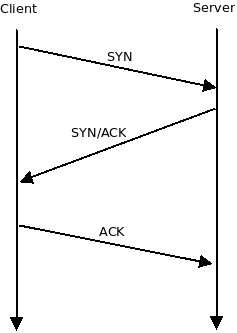
\includegraphics[scale=0.45]{3wh.png}
\caption{TCP Three-way handshake}
\label{fig:handshake}
\end{figure}

An interesting work presented a system for detecting abnormal traffic in a network, using a flow-based approach, extracting the traditional 5-tuple from the flow extractor \cite{kim2004flow}. The authors define the term abnormal as traffic that induces a malicious purpose, as is the case of the traffic generated by DoS/DDoS, worms or even scanning. Moreover, this work is particularly interesting as they focus their effort on detecting DoS/DDoS attacks, as we will be describing below.

Their detection model consists in two parts, namely flow header and traffic pattern detection modules. Whenever one of these two modules detects an attack, an alarm is triggered, indicating the network manager that an attack might be occurring, very much like a signature-based IDS would operate. The first module is in charge of inspecting the fields of the gathered flow headers. This allows to detect some flooding attacks that possess specific values, e.g. having Broadcast as the IP destination address. Table \ref{table:dos-fields} presents an extensive list of such values that will be validated and the respective attack that they might point out to. When validating the protocol fields, the detection is pretty straightforward, needing only to inspect the corresponding fields and check is they match or not, leading to a possible trigger. However, when referring to the packet count and flow size, the term \textit{large} is rather ambiguous, as they depend on the volume of traffic at the time, and the kind of traffic that is being produced. And so, to address this, this value is obtained by calculating a percentile threshold of the observed values.  


\begin{table}[]
\centering
\begin{tabular}{|c|c|c|}
\hline
\textbf{Protocol}     & \textbf{Fields}                                                                                                           & \textbf{Attack} \\ \hline
\multirow{3}{*}{ICMP} & \begin{tabular}[c]{@{}c@{}}Echo Request + \\ Destination IP = Broadcast\end{tabular}                                      & Smurf           \\ \cline{2-3} 
                      & Large Flow size or Packet Count                                                                                           & Ping of Death   \\ \cline{2-3} 
                      & Large Packet Count and Flow Size                                                                                          & ICMP Flooding   \\ \hline
\multirow{2}{*}{TCP}  & \begin{tabular}[c]{@{}c@{}}Source IP address = Destination IP address \\ or\\ Source Port = Destination Port\end{tabular} & Land            \\ \cline{2-3} 
                      & Large Packet Count and Flow Size                                                                                          & TCP Flooding    \\ \hline
\multirow{3}{*}{UDP}  & Destination/Source Port = Reflecting Port                                                                                 & Ping-Pong       \\ \cline{2-3} 
                      & \begin{tabular}[c]{@{}c@{}}Destination IP address = Broadcast\\ and\\ Destination Port = Reflecting Port\end{tabular}     & Fraggle         \\ \cline{2-3} 
                      & Large Packet Count and Flow Size                                                                                          & UDP Flooding    \\ \hline
\end{tabular}
\caption{Summary of fields in flow headers that can trigger attacks}
\label{table:dos-fields}
\end{table}

During a scan, an attacker makes a great amount of connection attempts, therefore generating many flows in which the packet count is small (approximately 40 bytes). If this scanning falls in the category of \textit{port scanning}, the attacker will sweep a great amount of port in the target host, therefore generating traffic in which the destination IP address is constant. However, if it is a \textit{network scanning}, the attacker will make many connections with many different destination IP addresses, searching for a service availability in one of them. With this said, we can conclude that both the total packet count and total bandwidth consumption can be either small or large, depending on the number of host connections and the number of ports, therefore making it impossible to use these two values to detect scanning attacks. Both Smurf and Fraggle attacks force traffic gathered by the victim, using a third party, which will create as many flows as the number of hosts in the third party used, consequently increasing both total packet count and total bandwidth consumption. And, because the number of repetitions of the transmission (being the destination address the Broadcast address) of spoofed packets determines the packet count for each flow, these parameters are also unavailable for detecting attacks.

The need for a second detection module derives from the fact that some attacks (and consequently, their patterns) can not be detected only by inspecting the flow headers fields and analyzing flows individually. In order to detect these, they need the traffic information capable of identifying patterns in it, and this can be achieved by aggregating related flows. From these aggregations, it is now possible to detect both flooding and scanning attacks (not only port scans, but also network scans), by checking the information sent and received from a host. They use two hash tables, in which the traffic pattern data aggregated for the same Destination or Source IP address is recorded. The detector checks if a large number of flows appears, the flow size of an individual flow is small, and also if the number of packets per flows is also small. If these conditions are verified, and if the number of distinct destination ports is high and the number of source IP address traffic generated is small, then the traffic is assumed to be a host scan. Else, if there is a small number of destination ports and a small fraction of the ratio $\frac{n(ACK)}{n(SYN)}$, it implies that we are in the presence of a TCP SYN flooding attack.


Another approach for detecting DoS attacks was done using 2D sketches. Not only this detects such attacks (their main focus relies on TCP SYN flooding detection), but also can cope with the detection of the various types of port scans \cite{Gao2006}. A sketch is an hash table used to quickly store information, mainly counting the occurrences of a given event. When this concept first came up, these hash tables had only one dimension, but the work presented by \cite{Gao2006} introduces the use of a two-dimensional table. With this data structure it is possible to characterized the observed traffic, in order to draw some conclusions, which in this case is the detection of port scans and DoS attacks.

As it was just mentioned, this system is able to detect both port scans (which is also extensible to detect most of large-scale worm propagations) and TCP SYN flooding attacks, using sketches as a base for statistical intrusion detection. To achieve so, each of the network routers (may be either edge or backbone routers) are configured to record network traffic into sketches. From the multiple created sketches (one for each router), they summarize all of them into one aggregated sketch, therefore allowing to distinguish from many different attacks observed. Then, they apply time series algorithms on these in order to obtain a forecast sketch, which will be used for the change detection. By subtracting this forecast sketch to the current one (i.e. in the present time), it is obtained a forecast error, which, if sufficiently large, indicates that there is an anomaly. By reversing the sketches, they obtain the key characteristics of the recorded flows, allowing to mitigate the attacks. In case of the values recorded trespass a certain defined threshold, the system triggers an alarm, indicating an attack.

The first step in their algorithm was to create a reversed sketch with keys $ {DIP,Dport} $ and whose feature is $ \#SYN - \#SYN/ACK $, which allows to detect SYN flooding attacks, as the attacker would be targeting a certain service in a specific destination port on a small set of hosts. The feature value $ \#SYN - \#SYN/ACK $ means that on every incoming SYN packet, the sketch entry would be incremented by one, and by every incoming SYN/ACK packet the sketch entry would be decremented by one. This set of DIPs will be stored in a set called $FLOODING\_DIP\_SET$, to be used in the following set. Then, another reversible sketch is to be applied, only this time with the keys $ {SIP,DIP} $, which could detect any intruder that was trying to attack a particular IP address. These attacks could either be a non-spoofed SYN flooding attack, or a vertical scan. With this data, the algorithm would then proceed to check if, for every pair in this sketch, the DIP is present in the $FLOODING\_DIP\_SET$,and if so, it would store the SIP in a set called $ \#SYN - \#SYN/ACK $. If not, this is the attackers IP address and this is considered a vertical scan. The third step was to use a reversible sketch with keys ${SIP,Dport}$ and feature values $ \#SYN - \#SYN/ACK $, once again. This allows to detect any large number of unfinished connections for a specific destination port. For each of ,the key pairs, it checks if the key SIP belongs to $ \#SYN - \#SYN/ACK $, and if so, concludes it is a non spoofed SYN flooding, and if not, it is a horizontal scan. After these three steps, the system then applies the time series analysis from which will result the error function used to detect anomalies. 


%%%%%%%%%%%%%%%%%%%%%%%%%%%%%%%%%%%%%%%%%%%%%%%%%%%%%%%%%%%%%%%%%%%%%%%%%%%%%%%
\subsubsection{Worms}
%%%%%%%%%%%%%%%%%%%%%%%%%%%%%%%%%%%%%%%%%%%%%%%%%%%%%%%%%%%%%%%%%%%%%%%%%%%%%%%
A \textit{worm} consists on a harmful software that, unlike the well-know case of a virus, has the capability to autonomously explore software vulnerabilities, thus making it capable of replicating itself throughout a network.

This specific attack is usually divided in two distinct phases: (i) a scanning phase, in which the worms probes several machines in order to find a vulnerability and then proceed to spread the infection; (ii) the transfer phase, in which the worm proceeds to send the harmful code and infect the victim. As the first phase is a well know case (as described above, in the \textit{port scanning} phase), the discovery of the scan can be crucial in identifying the attacker. Due to the fact that most of the network traffic relies on secure connections, and therefore the payload of traveling packets in most of the times is encrypted (e.g. TCP traffic), a major emphasis is given to the detection of the first phase, as is would be very difficult to detect malicious content of packets in a flow-based analysis. 

From using protocol graphs \cite{Collins2007}, to extending port scan detection approaches, to assigning hosts to sets of classes, many can be the strategies to identify \textit{worms} in a network, based on the analysis of network flows.  

The authors of \cite{Collins2007} developed a system capable both of detecting hit-list (a list of target servers that were previously identified) \textit{worms} and identifying bots (next section), using \emph{protocol graphs}. A protocol graph 
is a representation of traffic logs for one specific, in which its vertices (or nodes, as sometimes referred in literature) are representations of IP addresses and the edges are the connections existing between those two entities. The system's detection approach is based on graph size and largest connected component properties. The first is the total number of connected vertices, and the latter is the number of vertices in the largest connected component of the graph, i.e. the vertex with the most connections overall.

In that research, only four protocols were considered:
\begin{itemize}
	\item \textbf{HTTP}, identified by observing a connection in which one of the peers uses port 80 (either destination or source); this represents the majority of the traffic observed
	\item \textbf{SMTP}, identified by observing connections where one of the peers uses port 25; this is the second most active protocol producing traffic in the network
	\item \textbf{FTP}, which can be identified by observing the usage of port 20 by one of the entities in a connection
	\item \textbf{Oracle}, identified when one of the peers is using port 1521. As this protocol requires a login and password to authenticate an user, its expected that users connected to a smaller number of servers 
\end{itemize}


In order to construct the graph, flow records were extracted from Cisco NetFlow-enabled routers, in a large intercontinental network. These records were collected throughout a period of 5 days. 
As stated by the authors, many \textit{worm} detection systems  on the  detection of an unusual high number of frequent connections between peers, and track them by inspecting connection evidences such as \textit{half-open} TCP connections. So, to avoid this issue, the attackers can use \textit{hit lists}, which consists in a list of previously identified servers. Using this, they need not to contact random servers across the network and can focus on these known ones, making it harder for the systems to detect this scanning phase. 

The detection model consists in the hypothesis that an attacker that contacts different servers through a hit list will affect the graph in two ways (as depicted in Figure 2): first, when an attacker is communicating with servers that were not active during the observation period $\pi$, there will be a \textit{graph inflation}, i.e. there will be an increase in the number of vertices in the graph. The other way is when the attacker communicates with already active servers in the observation period $\pi$, and this will affect the \textit{component inflation}, i.e. increasing the number of connections in one vertice.The system will raise an alarm whenever one of two conditions are verified:
\begin{enumerate}
\item The total size of the graph is bigger than its mean value in the observation period $\pi$ along with its standart deviation over time
\item The largest component size is bigger than its mean value in the observation period $\pi$ along with its standart deviation over time
\end{enumerate}

\begin{figure}[htp]
\centering
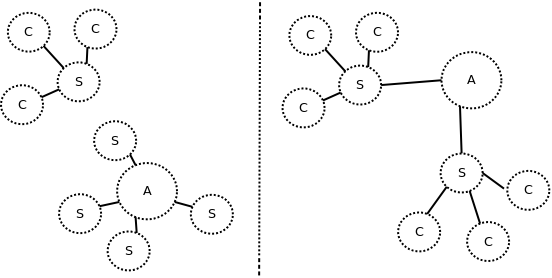
\includegraphics[scale=0.3]{g_inflations.png}
\caption{Graph inflation in the left side and component inflation on the right side}
\label{2}
\end{figure}

By observing the two previously mentioned possible inflation in the graph, they were able to detect when an attack is on course, given that the first hypothesis will raise a trigger for condition (1) - a \textit{graph inflation} will result in a considerably relevant increase of the total graph size, and the second hypothesis will raise a trigger for condition (2) - the \textit{component inflation} reflects a big increase of the largest component size value.

One other, simpler, approach to detecting network worms was addressed by Dubendorfer \textit{et al.} \cite{wormFramework}. This came with the development of their framework for both worm attack detection in real-time and the network backbone monitoring, UPFrame. In this framework, they developed algorithms for host behavior, network activity and traffic characterization for attack detection.

The host behavior detection module is the one used to identify worms in the network. The hosts are assigned to a set of classes, and this is updated periodically (in the paper the defined interval was 1 minute). However, host will only belong to one of these classes if it presents an unusual behavior, only belonging to any of them when a certain threshold is trespassed (note that they are not restricted to belong to only one class, can belong to more than can). This leads to the concluding that the rapid change in the cardinality of a set indicates a significant change in the network behavior. The classes are the following:

\begin{itemize}
\item \textit{Traffic}, for hosts with $\frac{bytes\_send}{bytes\_received} > 3 $
\item \textit{Connector}, for hosts with $ \#outgoing\_connections > 10 $
\item \textit{Responder}, for hosts with $ \#bidirectional\_connections > 1 $ 
\end{itemize}


The hosts in the \textit{Traffic} class are the one that send much more traffic than what they receive. This is the kind of behavior that is expected for code exploiting worms or worms that spread on email attachments, for example \cite{Dubendorfer2005}. The hosts in \textit{Responders} are those that maintain bidirectional connections, which the author define as flow in opposite directions between a pair of hosts, that are spaced from each other in less than 50 ms. Hosts that respond to TCP scans are usually in this class. And, at last, hosts in \textit{Connector} are those that initiate many outgoing connection without maintaining a bidirectional connection, which is the typical behavior for a scanning. With the definition of these classes, the attack detection is based on the assumption that if a host tries to infect others during a worm outbreak, the behavior of many hosts will change, causing great variation in the cardinality of the sets. 

%%%%%%%%%%%%%%%%%%%%%%%%%%%%%%%%%%%%%%%%%%%%%%%%%%%%%%%%%%%%%%%%%%%%%%%%%%%%%%%
\subsubsection{Botnets}
%%%%%%%%%%%%%%%%%%%%%%%%%%%%%%%%%%%%%%%%%%%%%%%%%%%%%%%%%%%%%%%%%%%%%%%%%%%%%%%

A \textit{botnet} is network an infected hosts (referred to as \textit{bots}), that is controlled by an entity (referred to as \textit{master} or \textit{botmaster}). The master controls its bots through a command and control - C\&C - infrastructure, and uses them as a third party to launch attacks and intrusions in the network, such as spam, phishing, DDoS and identity theft. This C\&C infrastructure could either be an IRC (Internet Relay Chat) channel, or an HTTP server. 

Botnets are considered to the date as one of the biggest security threats, and the most difficult to detect, as the \textit{botmaster} is not easy to identify, and requires a long period of observation. However, by identifying it, most of the problem is solved \cite{Sperotto2010}. 


An important contribution to this field was made by Zeng \textit{et al.} \cite{Zeng2010}, who developed a protocol-independent framework to detect botnets, using both host-level and network-level information. They constructed their detection model based on the fact that bots within the same botnet are likely to receive the same input from their botmaster and to take similar action, while benign hosts are seldom to behave as such. The system architecture can be divided in three parts: 
\begin{enumerate*}
\item Host analyzer;
\item Network analyzer;
\item Correlation engine;
\end{enumerate*}.

The first part can be broke down in two modules:
\begin{enumerate*}
\item In-host monitor;
\item Suspicion-level generator
\end{enumerate*}. The first one monitors in run-time the host behavior. By studying contemporary botnets, the authors found that these act in three different sectors in the hosts: the registry, the file system, and the network stack. When a computer is infected (note that this study refers only to Windows operating systems), the botnet begins by generating an \emph{exe} or \emph{dll} file in the system directory. Then, it registers an autorun key in registry to run automatically when system boots. Also it injects its code into other processes in order to hide its presence, and disables any anti-virus software and task manager, if needed, and may open one or more ports for further communication, establishing connections with botmaster or peers in order to launch its attacks. The combination and aggregation of these mentioned behaviors is a strong indicator that the host might be infected. This run-time behavior is transformed into a \textit{behavior vector}, consisting of 9 features. All together are intrinsic to a botnet behavior. As the network analyzer is able to gather network-level information, the in-host analyzer need to focus on aspects the can't be observed externally, and also features that can, and so the network stack features like Number of Suspicious Ports used, Number of Unique IP addresses contacted and Number of SMTP Flows are accounted. The suspicion-level generator uses a Support Vector Machine, a supervised machine learning algorithm to quantify the suspicion level. The training data fed to the system consists in both benign and malicious behavior profiles. Based on this training process, a hyperplane is created, which will correspond the the classification. When a new behavior vector arrives, the Support Vector Machine will compute its distance from the hyperplane, and decide whether to classify it as a benign or a malicious behavior. 

The second part of the system architecture is also divided in two parts: 
\begin{enumerate*}
\item flow analyzer;
\item clustering module
\end{enumerate*}. The flow analyzer flow data as input, and begins filtering it. This filtering process consists in removing internal and legitimate flows, which is the traffic within the network and traffic to well known destinations, respectively. Then, it processes the remaining flow records of all hosts in a network to extract trigger-action patterns of interest in each time interval. As stated previously, bots receive the same input, and so, the analyzer looks for suspicious flow with the same destination IP address and transport protocol across all hosts, and labels them as triggering flows. Once again, by studying contemporary botnets, the authors found that bots usually connect to same group of C\&C servers or peers to communicate with their \textit{botmaster}, and execute the commands immediately. As the benign hosts rarely visit same IP with same protocol, upon filtering legitimate and internal flows, it is possible to distinguish them from the infected ones. From the observed traffic, 17 flow features are extracted into a feature vector. The first 14 are for classifying traffic pattern, and last 3, which are common to those also extracted from in-host monitoring, are used to measure botnet's malicious intent to some degree. Then, a hierarchical clustering algorithm is used upon these feature values for each time interval, in order to group hosts that might be considered botnets. 

After all this data is extracted both from the network analyzer and the in-host analyzer, the correlation engine performs a last analysis to check if a botnet is or not present. When a group of hosts are clustered, the respective host analyzers are requested the suspicion-level together with some network statistic. There are two possible outcomes from this step: 
\begin{enumerate}
\item the network statistics sent from the in-host analyzer may differ from those observed by the network analyzer, implying that the host if sending falsified data, therefore triggering immediately an alarm
\item If the results are consistent from both analysis, then the suspicion-level and clustering quality must be analyzed by the correlator. This is done by a function with two parameters. The first is the suspicion-level, which itself is a quantitative measure. The second is the distance between the hosts presented in the same cluster, which is computed by a simple Euclidean Distance. 
\end{enumerate}

With these three modules, the authors managed to track, from real-world data, different kinks of botnets, achieving low false-positive and false-negative rates. 

%%%%%%%%%%%%%%%%%%%%%%%%%%%%%%%%%%%%%%%%%%%%%%%%%%%%%%%%%%%%%%%%%%%%%
\subsection{Intrusion Detection based on Machine Learning}\label{ssec:mlearning}
%%%%%%%%%%%%%%%%%%%%%%%%%%%%%%%%%%%%%%%%%%%%%%%%%%%%%%%%%%%%%%%%%%%%%%%%%%%%%%%
A increasing trend in intrusion detection systems is the use of machine learning techniques \cite{Pitts2014, Sperotto2010}.

\emph{Machine Learning} can be defined as a collection of methods that aim to attain knowledge, by building an intelligent system through the observation of pattern in a given environment \cite{Pitts2014}. This knowledge is refined and improved at each iteration, by learning from previous experiences and observations. As expected, such method has been used in an enormous number of different applications, in many different fields of science, such as natural language processing, speech recognition, bioinformatics, spam detection, network intrusion, among many others. 

Machine learning algorithms can be divided into two major fields:

\begin{itemize}
\item Supervised learning
\item Unsupervised learning
\end{itemize}

The first one relies on a labeled training dataset for the system. The dataset consists in an extensive list of input data that aims to train the system, making correspondences between keywords and their meaning or interpretation that is expected to the system. After this training phase, the system is ready to classify data based on the training set it was trained to. Examples of this method are the algorithms Na\"{i}ve Bayes and Support Vector Machine. While Supervised methods relies initially on the introduction of training data, Unsupervised methods only receives as input a feature vector without any kind of labeling, and is used to means such as discovering similar groups within a data set. Clustering is an example of this kind of learning. 

In the field of network intrusion detection, machine learning has been able to classify network traffic and identify both anomalous patterns and potentially harmful users. When it comes to embed this technology in an Intrusion Detection Systems, generally this is the strategy adopted:

\begin{itemize}
  \item \textit{Anomaly-based detection} (or \textit{behavior-based}), in which normal traffic patterns are differentiated from anomalous ones. It focuses its attention on finding patterns that would not be expected from the user's behavior. Unlike \textit{misuse-based} IDSs, these patterns are unknown to the system
\end{itemize}

These two make up the classical approaches, being that machine learning is applied to the \textit{anomaly-based} approach, rather than the \textit{misuse-based} one. However, there are some variants to these, as we will now be discussing.
Eskin \textit{et al.} were one of the first to address unsupervised learning in intrusion detection systems \cite{LeonidPortnoy}. They present a new technique, which they entitle \textit{unsupervised anomaly detection}. This technique allows to train the system with a set a dataset of completely unlabeled data, providing the chance of detecting unknown attacks to the network, which would not be possible when training the system with labeled data - in this case, the system is only able to recognize those labeled intrusions; and also, the manual classification of data can be very hard and tiresome.
They used the famous KDD99 dataset for the training of the system. This dataset is a labeled dataset that was built in a military environment, and is provided to the intrusion detection research community (note that nowadays this dataset is almost deprecated, as it was collected in 1999). The features were extracted from connection record the raw data gathered throughout the simulated intrusions present in the dataset. This included features such as the basic components of a TCP connection (duration time, protocol type, etc.), some others that were not so trivially obtained (number of file creation operations, number of failed login attempts, etc.), and some other features captured in a small two-second time windows (number of connections to the same host as the current connection in this timespan, percentage of connections that have \textit{SYN} and \textit{REJ} errors, etc.). All summed up, the authors considered a total of 49 features. Also, the dataset was filtered, so that there would only exist a percentage of 1 to 1.5\% of attacks vs. 98.5 to 99\% normal traffic instances. This is done because of the need of the system to learn to distinguish intrusion instances from the normal ones, and the original dataset was composed mainly of intrusions.

Their solution was based on two assumptions:
\begin{enumerate}
  \item The number of normal instances greatly outnumbers from the number of intrusions
  \item The intrusions themselves are qualitatively different from the normal instances
\end{enumerate}

The system clusters the collected data through an algorithm that computes a distance-based metric. However, because of the different distributions that each feature vector may have, these have to be normalized in order to apply the same metric to all of the vectors. After computing the clustering algorithm, these new clusters can now be classified as being normal traffic instances or an intrusion. The first assumption implies that small clusters correspond to the intrusion instances, as opposed to the bigger clusters that represent normal instances; the second assumption implies that normal and intrusion instances will not be under the same clusters because of their qualitative differences.


In order to measure the performance of the system, they used the following metrics:
\begin{itemize}
\item \textit{Detection rate}, which represents that ratio of intrusions detected by the system, by the intrusions present in the dataset
\item \textit{False positives}, which is the ratio of the total number of intrusions that were incorrectly detected by the system, by the total number of normal instances
\end{itemize}

In this solution, there is an inevitable trade off between these two indicators, as one scales with the other. However, they managed to obtained a fairly reasonable ratio of \textit{detection rate} and \textit{false positives}.

This paper presents mainly two advantages to the traditional intrusion detection systems. The first, is that it does not require any kind of manual classification, and the second is that the system is capable of detect intrusion that were previously unknown.

Similar to this work, and more recently, was developed a system that goes by the name of UNIDS (Unsupervised Network Intrusion Detection System) \cite{Casas2012}, which is able to detect unknown attacks without requiring any labeling, signatures or training. In order to understand the results obtained, they always rely on the assumption, just like the previously stated work, that the vast majority of the observed traffic is considered normal, rather than anomalous. 

From a higher level perspective, the architecture of the solution can be divided in the main components:
\begin{enumerate*}
\item the detection of \emph{anomalous time slots}, resorting to \emph{change-detection algorithms};
\item the processing of the flow records present in the identified anomalous time slots, creating clusters of the gathered data;
\item the ranking of outliers generated from the clustering algorithm 
\end{enumerate*}
%%%%%%%%%%%%%%%%%%%%%%%%%%%%%%%%%%%%%%%%%%%%%%%%%%%%%%


In the first part of the solution, upon the extraction of network flow records - which are 5-tuples: the source and destination IP addresses and ports, and the protocol used - these are aggregated by unique \textit{aggregation keys} ($ l_{i}$):
\begin{enumerate*}
\item traffic per time slot ($ l_{1} $);
\item source network prefixes (IP source /8, /16, /24) ($ l_{2-4} $);
\item destination network prefixes (IP destination /8, /16, /24) ($ l_{5-7} $);
\item source IP addresses ($ l_{8} $);
\item destination IP addresses ($ l_{9} $)
\end{enumerate*}. The first seven are used exclusively to the change-detection phase, while the last two are used on the clustering algorithm. In order to detect anomalous time-slots, they construct time-series $ Z_{i}^t $ for traffic metrics like the number of packets and IP flows per time slot. For each time slot, a change-detection algorithm is used to analyze the different time-series associated with each one of the aggregation keys (from $ l_{1} $ to $ l_{7} $), and the respective time slot is considered to anomalous if the change-detection algorithm triggers an alarm for any of the defined traffic metrics. The fact that multiple aggregation levels are being used, allows them to have a higher reliability, since they are able to analyze different perspectives of the traffic, going from finer to more coarse aggregation levels. 

Upon the discovery of the anomalous time slot, the \emph{abnormality degree}  will be calculated for each and every one of them, using both clustering and outliers analysis techniques. An outlier is any sample that does not belong to a cluster, and these will correspond to the anomalies in the traffic, due to the assumption that the vast majority of the observed traffic is normal. The traffic anomalies can be grouped in two different classes: the first one is a \textit{1-to-N} anomaly, in which an IP flow from a single source infects $N$ target hosts, and such is the case of \textit{port scans}, \textit{worms} and \textit{viruses}. The other one is \textit{N-to-1}, which, analogous to the previous one, has IP flows from $N$ sources infecting one single destination. The aggregation key $l_{8}$ (IPsrc) allows to identify the first class, while $l_{9}$ allow to identify the latter. 

Each of the aggregated flows is described by $x_{i} \in \mathbb{R}^m $, a set of $m$ traffic features, such as the number of sources or destination ports, and a component of $ X \in \mathbb{R}^{m \times n}$, the complete matrix of all the features, being $n$ the number of aggregated flows. The previously mentioned clustering algorithm will be performed the feature space $X$. First, an algorithm called Sub-Space Clustering will be applied to create $N$ data partitions $X_{i}$ out of $X$, by selecting $k$ features from the complete set of $m$ features. From these partitions, another clustering algorithm called Density-Based Clustering will be applied to each one of them, generating partitions $P_{i}$. Apart from the partitions, there will also be generated the previously mentioned outliers, which will later on be ranked in order to find classify the anomalies. To this, they use the concept of Evidence Accumulation, which uses the clustering results of the multiple partitions, and produces similarity measures that are able to better reflect their groupings. 

Now that we have presented a couple of unsupervised network IDSs, we present one that is built in a supervised fashion. Winter \textit{et al.} \cite{Winter2011} developed a system that trains the network data with a One-Class Support Vector Machine (OC-SVM) algorithm. 

Based on the fact that machine learning methods achieve better results when classifying inliers than when classifying outliers, the training set consisted only in malicious data, rather than benign data. This way, the inliers will the be the malicious data, for which the training algorithm will achieve better results. The first step in their system was, upon the receiving of a flow stream, the processing of data. In this step, they filter the flows from the dataset in order to achieve a feasible value that would not overload the learning process. Then, they needed to tune the OC-SVM, in order to achieve the best results possible (in this case, the false negative and miss rate were taken into account). To do so, they needed to achieve the best trade off between the parameters $v$ and $\gamma$ , which will determine the fraction of outliers in the set and the width of the RBF (Radial Basis Kernel) - that was added to the algorithm, respectively. Also, in this step, the most valuable features will be selected. This optimization was done first in a coarse grained fashion, to determine the best feature subset and the best trade off between the two parameters; and then, in a finer grained fashion, that would further explore the relation between the two parameters to achieve better results. From this optimization, the most relevant attributes were: Packets per Flow, Source Port, Destination Port, TCP flags and the IP protocol.

With this setup, they managed to achieve a 0\% false alarm rate, and a miss rate of only 2\%, approximately. This shows that this approach might be interesting to consider to our solution, as the results obtained were extremely good. 
 
%%%%%%%%%%%%%%%%%%%%%%%%%%%%%%%%%%%%%%%%%%%%%%%%%%%%%%%%%%%%%%%%%%%%%%%%%%%%%%%
\section{Overview of the proposal}\label{sec:arch}
%%%%%%%%%%%%%%%%%%%%%%%%%%%%%%%%%%%%%%%%%%%%%%%%%%%%%%%%%%%%%%%%%%%%%%%%%%%%%%%

In this section we describe a flow-based Network Intrusion Detection System capable of detecting unknown attacks. 
This section starts with an overview of the system idea, followed by the
architecture of the solution, proceeding to a more detailed view of each module. Besides, this
chapter provides a description of the new ideas introduced and to be further implemented.

This works aims to cover two major drawbacks of traditional NIDSs:
\begin{enumerate}
\item The inability to react to an unknown pattern
\item The slow processing and analysis of the traffic payload, as well as inability to interpret its content
\end{enumerate}

The first drawback may be countered by using an unsupervised machine learning algorithm, and the second is overcome by performing the analysis at a flow-level. Combining these two concepts we are able to design such a system that overcomes these issues. 

\begin{figure}[htp]
\centering
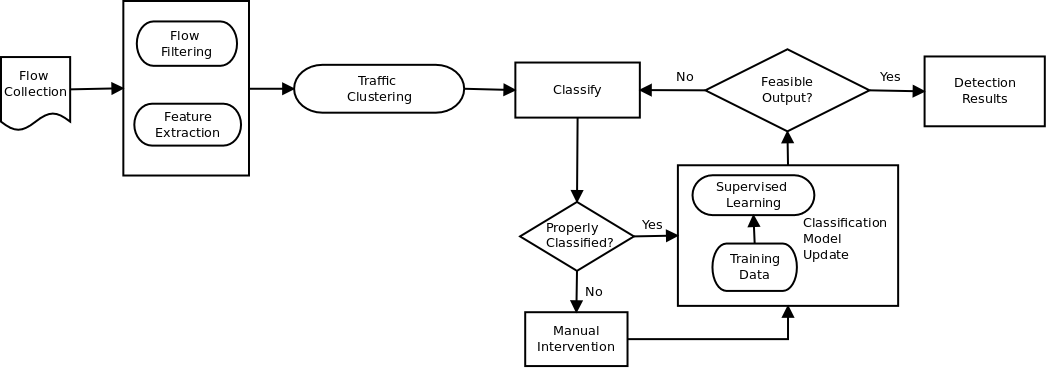
\includegraphics[scale=0.2]{solution.png}
\caption{Solution's architecture}
\label{fig:sol}
\end{figure}




First of all, upon the receiving of the gathered flow, it will be performed a filtering on it. This filtering will consist in removing internal traffic and legitimate traffic, i.e. the traffic whose destinations are well-know, as described in \cite{Zeng2010}, as it will reduce significantly the number of cases for the system to compute. Then, the system will begin by extracting 5-tuples from the raw flow data, and aggregate them by source and destination IP address. These 5-tuples will be fed to the clustering algorithm, that will create groups of hosts that share a common pattern. It will be taken into account the assumption that the majority of the observed traffic is benign rather than malicious. With this said, there will then be a manual intervention on the outliers produced by the latter algorithm, in order to better perceive the characteristics of this traffic, leading to the production of a labeled dataset that will serve as training for the next step. The system will be running a supervised learning algorithm that will proceed to classify the traffic that was perceived as outliers by the clustering algorithm. Upon this classification, the system should be able to correctly identify the observed  malicious traffic. Figure \ref{fig:sol} provides a clearer view for this idea.


The first step - filtering and feature extraction - will be crucial for the performance of the whole system, as it will be the input for the rest of it. If carefully chose, the system may be able to produce good results, performing an accurate clustering of data; if not, the clustering result might be completely inconclusive, thereby impairing the remaining modules. The 5-tuple was selected as it is the most generic set of features, and with it almost every common intrusion may be detected. Furthermore of decision of using aggregated flows rather than simply analyzing individual flows, was due to the observation made throughout the study of existing contributions in the intrusion detection community \cite{Casas2012,schatzmann2011fact,Sadre2012,kim2004flow} that aggregated flows provide a more precise analysis, e.g. in the case of detecting DDoS. Some attacks, if were to be analyzed using individual flows, would be much harder to detect. The choice of using the source and destination IP addresses as aggregation keys was inspired by \cite{Casas2012}, that used them to distinguish groups of \textit{1-N} and \textit{N-to-1} anomalies. 

On these aggregated features it will be applied the unsupervised clustering algorithm, that will proceed to form various large groups of hosts, and some outliers. According to the previously mentioned assumption, these outlier will represent the intrusions in the network, and it is of utmost importance to analyze them. In a first run of the system, the supervised learning module has not yet any knowledge at all, and so there is a need for a manual intervention that will classify and label these outliers. This manual classification will serve as input to the supervised learning algorithm, that, over time, will come more and more capable of classifying on its own. In the following runs, there may not be a need for manual intervention if the classification produced by this learning algorithm is feasible (which is to be validated with ground truth, as will be discussed in the next section); else, an expert classify this traffic manually and feed the algorithm once again. The supervised learning algorithm that we will be using is yet to be studied in order to choose the best possible fit, being however the Support Vector Machine a possibility, as it is studied in the previous section, and has already proven that it can achieve satisfying results. Other possible algorithm for this purpose might be a Decision Tree. For the unsupervised learning we will use, as previously mentioned, a clustering algorithm. However, there are many kinds of different clustering algorithms, capable of identifying different forms and shapes \cite{Casas2012}, and therefore we will also study which algorithm better fits our IDS. If tuned correctly, these will be able to correctly inform the network manager if an intrusion is occurring, therefore satisfying our goal.

%%%%%%%%%%%%%%%%%%%%%%%%%%%%%%%%%%%%%%%%%%%%%%%%%%%%%%%%%%%%%%%%%%%%%%%%%%%%%%%
\section{Evaluation}\label{sec:eval}
%%%%%%%%%%%%%%%%%%%%%%%%%%%%%%%%%%%%%%%%%%%%%%%%%%%%%%%%%%%%%%%%%%%%%%%%%%%%%%%

This system's performance will be validated mainly with real-world data from Vodafone Portugal, which will provide a collection of data gathered throughout two weeks. 

Prior to analyzing this set, the following steps will be performed:
\begin{enumerate}
\item Run the system on an intrusion-free dataset from SiLK \cite{silk}
\item Manually inject intrusions in this dataset, and run the system once again 
\end{enumerate}

The idea from these two steps is to begin by checking if in an intrusion-free environment the system indeed does not detect any intrusion, thus revealing that the system is free of false positives. With the injection of some intrusion in that same dataset, the system should be able to detect them, thereby indicating that in the presence of intrusions, the system is capable of detecting them. These two steps will be a ground-truth validation, as we know \textit{a priori} what is and is not an intrusion, and are able to check if the system behaves correctly. Upon these two validations, we will run the system in the real-world data traces from Vodafone Portugal, and study its performance results.

We will be looking for two evaluation metrics:
\begin{enumerate}
\item \textit{False positive rate}
\item \textit{False negative rate}
\end{enumerate}

The first one will indicate if the system is perceiving perfectly benign data as intrusions, which is obviously not wanted, as it might mislead the network managers. The second one indicates how many intrusions the system was not able to detect. There will be a trade off between these two metric, as we will be focusing on tuning the system as efficiently as possible. 


%%%%%%%%%%%%%%%%%%%%%%%%%%%%%%%%%%%%%%%%%%%%%%%%%%%%%%%%%%%%%%%%%%%%%%%%%%%%%%%
\section{Scheduling of Future Work}\label{sec:schedule}
%%%%%%%%%%%%%%%%%%%%%%%%%%%%%%%%%%%%%%%%%%%%%%%%%%%%%%%%%%%%%%%%%%%%%%%%%%%%%%%

The scheduling of tasks for the future will be performed as follows:

\begin{itemize}
\item 19/01 - 22/03  -> Implementation of the proposed solution
\item 22/03 - 12/05 -> Experimental evaluation and tuning 
\item 13/05 - 04/06 -> Write a paper of this subject
\item 05/06 - 07/07 -> Write dissertation
\item 08/07 -> Deliver MSc Dissertation
\end{itemize}

%%%%%%%%%%%%%%%%%%%%%%%%%%%%%%%%%%%%%%%%%%%%%%%%%%%%%%%%%%%%%%%%%%%%%%%%%%%%%%%
\section{Conclusion}\label{sec:conclusion}
%%%%%%%%%%%%%%%%%%%%%%%%%%%%%%%%%%%%%%%%%%%%%%%%%%%%%%%%%%%%%%%%%%%%%%%%%%%%%%%

The main goal of this work was to present a system that would be capable of detecting network intrusions without requiring previous knowledge about what we were looking for. This documents begins by presenting a detailed overview of contributions on flow-based approaches to detect network intrusions, as well a a brief explanation of the concepts that surround and involve them, and the most commonly addressed intrusions, such as DoS, port scanning, worms and botnets. A possible NIDS capable of detecting these and other intrusion without having any \textit{a priori} knowledge is whereby proposed and discussed. Then, we also propose a set of metrics that will be able to correctly express the performance of the system.



%%%%%%%%%%%%%%%%%%%%%%%%%%%%%%%%%%%%%%%%%%%%%%%%%%%%%%%%%%%%%%%%%%%%%%%%%%%%%%%
\bibliographystyle{splncs03}
\bibliography{paper}
%%%%%%%%%%%%%%%%%%%%%%%%%%%%%%%%%%%%%%%%%%%%%%%%%%%%%%%%%%%%%%%%%%%%%%%%%%%%%%%

\end{document}
